We can also check the performance with this quantity that encompasses both the fidelity as well as the robustness of a protcol.
We are going to define the following quantity
\begin{equation}
	\eta = \sqrt{(1-F)^{2} + R^{2}}
	\label{eq:Sensitivity}
\end{equation}
where $F$ is the fidelity and $ R $  is the robustness.
The results are shown in the following plots for different number of particles and for different eSTA.

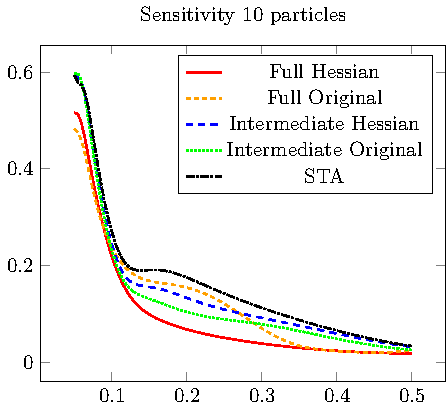
\includegraphics{./gfx/sensitivity_np10_nlambda5.pdf}
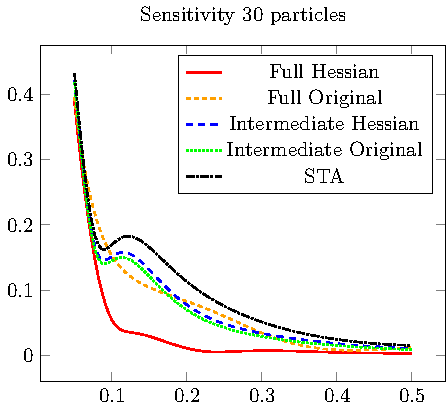
\includegraphics{./gfx/sensitivity_np30_nlambda5.pdf}

\begin{center}
 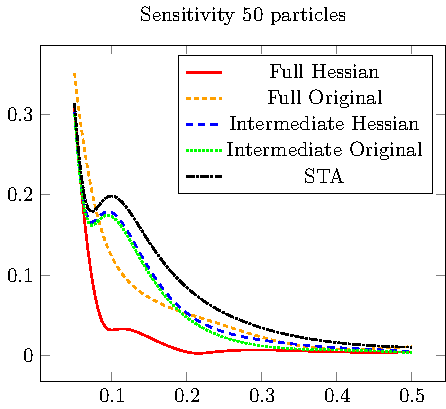
\includegraphics{./gfx/sensitivity_np50_nlambda5.pdf}
\end{center}



Again we can see that the best performances are achieved by the Hessian version of the eSTA protocol when applied to the full Hamiltonian of the system.

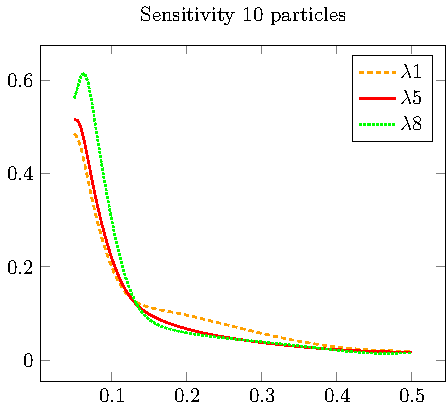
\includegraphics{./gfx/sensitivity_compare10.pdf}
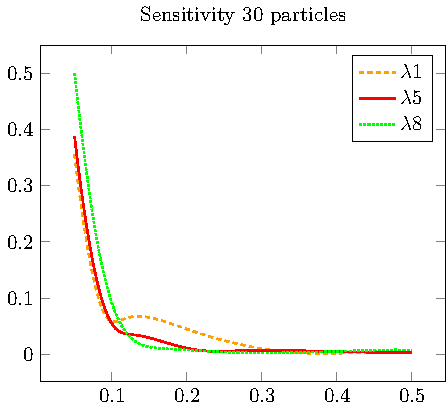
\includegraphics{./gfx/sensitivity_compare30.pdf}

\begin{center}
 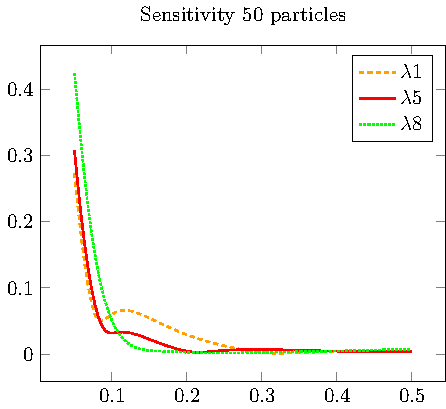
\includegraphics{./gfx/sensitivity_compare50.pdf}
\end{center}


Unsurprisingly, increasing the number of 
